\section{Цель работы}
Освоение процедуры синтеза адаптивного наблюдателя линейного объекта.


\section{Теоретические сведения}
На основе результата, полученного в лабораторной работе №5, рассматривается задача адаптивного наблюдения вектора состояния параметрически неопределенного линейного объекта.

Рассматриваемая задача состоит в построении оценки вектора состояния $\hat{x}$ такой, что
\begin{equation}\label{goal}
	\lim_{t \to \infty}{x(t) - \hat{x}(t)} = 0
\end{equation}

Cинтезируемый адаптивный наблюдатель должен одновременно оценить неизвестные параметры объекта управления $\theta$, а также построить оценку вектора состояния $\hat{x}$.

\section{Исходные данные}
Варианту \textnumero2 соответствует следующий набор исходных данных:
\begin{equation}
    a_1 = 2,
    \quad
    a_0 = 1,
    \quad
    b_1 = 1,
    \quad
    b_0 = 3,
    \quad
    k_1 = \sqrt{0.02},
    \quad
    k_0 = 0.01,
    \quad
    u = \sin{t} + 0.5 \cos{2t}
\end{equation}


\section{Результаты расчетов и моделирования}
\subsection{Модели исходного объекта}
Модель рассматриваемого объекта в форме ВСВ:
\begin{align}
    & \dot{x} = Ax + bu, \label{eq_state_space_model_of_plant}\\
    & y = Cx,
\end{align}
где
\begin{equation}
    A =
    \begin{bmatrix}
        -a_1 & 1 \\
        -a_0 & 0
    \end{bmatrix}\!\!,
    \qquad
    b = 
    \begin{bmatrix}
        b_1 \\ b_0
    \end{bmatrix}\!\!,
    \qquad
    C =
    \begin{bmatrix}
        1 & 0
    \end{bmatrix}\!\!\ldotp
\end{equation}

\subsection{Параметризация относительно выходной переменной}
Модель рассматриваемого объекта в форме ВСВ:
\begin{equation}
    \ddot{y} + a_1 \dot{y} + a_0 y = b_1 \dot{u} + b_0 u
\end{equation}
После применения к правой и левой частям этого уравнения оператора
\begin{equation}
    H(s) = \frac{1}{K(s)},
\end{equation}
где $K(s) = s^2 + k_1 s + k_0$ и некоторого количества алгебраических преобразований достигается следующий результат:
\begin{gather}
    \frac{1}{K(s)}[\ddot{y} + a_1 \dot{y} + a_0 y] = \frac{1}{K(s)}[b_1 \dot{u} + b_0 u] \\
    %
    \frac{1}{K(s)}[\ddot{y}] + a_1 \frac{1}{K(s)}[\dot{y}] + a_0\frac{1}{K(s)}[y] = b_1 \frac{1}{K(s)}[\dot{u}] + b_0\frac{1}{K(s)}[u] \\
    %
    \frac{s^2}{K(s)}[y] + a_1 \frac{s}{K(s)}[y] + a_0\frac{1}{K(s)}[y] = b_1 \frac{s}{K(s)}[u] + b_0\frac{1}{K(s)}[u] \\
    %
    \frac{s^2 \pm (k_1 s + k_0)}{K(s)}[y] = -a_1 \frac{s}{K(s)}[y] - a_0\frac{1}{K(s)}[y] + b_1 \frac{s}{K(s)}[u] + b_0\frac{1}{K(s)}[u] \\
    %
    y = \frac{k_1 s + k_0}{K(s)}[y] -a_1 \frac{s}{K(s)}[y] - a_0\frac{1}{K(s)}[y] + b_1 \frac{s}{K(s)}[u] + b_0\frac{1}{K(s)}[u] \\
    %
    y = (k_1 - a_1) \underbrace{\frac{s}{K(s)}[y]}_{\xi_2} + (k_0 - a_0) \underbrace{\frac{1}{K(s)}[y]}_{\xi_1} + b_1 \underbrace{\frac{s}{K(s)}[u]}_{\nu_2} + b_0 \underbrace{\frac{1}{K(s)}[u]}_{\nu_1} \\
    %
    y = \theta^T \omega,
\end{gather}
где
\begin{equation}
    \theta^T =
    \begin{bmatrix}
        k_1 - a_1 & k_0 - a_0 & b_1 & b_0
    \end{bmatrix}\!\!,
    \qquad
    \omega^T =
    \begin{bmatrix}
        \xi_2 & \xi_1 & \nu_2 & \nu_1
    \end{bmatrix}
\end{equation}

Параметризованная модель ОУ принимает вид:
\begin{equation}
	y = \theta^T \omega
\end{equation}

Заменим	параметры $\theta$ на оценки $\hat{\theta}$ и сформируем настраиваемую модель объекта:
\begin{equation}
\hat{y} = \hat\theta^T \omega,
\end{equation}
где $\hat{y}$ оценка переменной  $y$. 

Введем в рассмотрение ошибку:
\begin{equation}
	\varepsilon = y - \hat{y}.
\end{equation}

В итоге получим:
\begin{equation}
	\varepsilon = \tilde{\theta}^T \omega,
\end{equation}
где $\tilde{\theta}$~--- вектор параметрических ошибок.

Алгоритм адаптации:
\begin{equation}\label{aa}
	\dot{\hat{\theta}} = \gamma \omega \varepsilon,
\end{equation}
где $\gamma > 0$~--- коэффициент адаптации.

\subsection{Параметризация относительно вектора состояния}
После применения к уравнению~\eqref{eq_state_space_model_of_plant} матричной передаточной функции
\begin{equation}
\Phi(s) = (sI - A_0)^{-1},
\end{equation}
где
\begin{equation}
A_0 =
\begin{bmatrix}
-k_1 & 1 \\
-k_0 & 0
\end{bmatrix} \!\!,
\end{equation}
достигается следующий результат:
\begin{gather}
x = \sum_{j=0}^{1} \theta_{2-j} \Phi(s) e_{2-j} [y] + \sum_{j=0}^{1} \theta_{4-j} \Phi(s) e_{2-j} [u],
\end{gather}
где $e_i^T = [0\;0\;\ldots\;0\;\underbrace{1}_{i-th}\;0\;\ldots\;0]$.

Заменив тут параметры $\theta$ на их оценки $\hat{\theta}$, получим:
\begin{equation}
	\hat{x} = \sum_{j=0}^{1} \hat\theta_{2-j} \Phi(s) e_{2-j} [y] + \sum_{j=0}^{1} \hat\theta_{4-j} \Phi(s) e_{2-j} [u],
\end{equation}


Моделирование проводилось в течение около $20$ тыс. секунд, в связи с этим, для наглядности развития процесса, приводятся только первые 100 секунд моделирования и последние.

Было произведено два эксперимента. Во втором эксперименте увеличили количество гармоник сигнала $u$:
\begin{enumerate}
	\item $u = \sin{t} + 0.5 \cos{2 t}$;
	\item $u = 10 \sin{t} + 5 \cos{2 t} + 4 \cos{4 t} + 3 \cos{8 t}$.
\end{enumerate}
\begin{figure}[h]
    \centering
    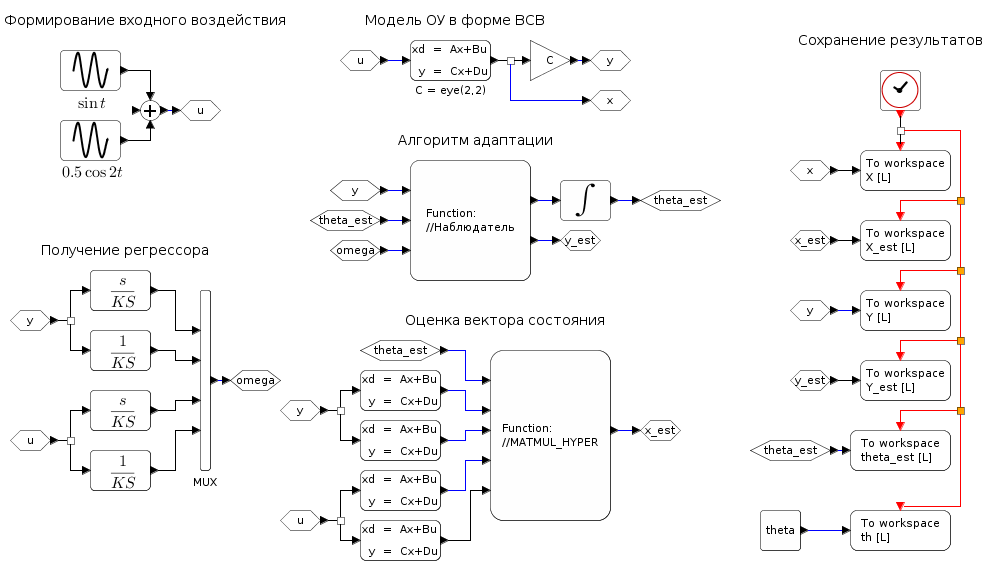
\includegraphics[width=\textwidth]{adapt_observer_1.png}
    \caption{Схема моделирования, применяемая для проверки работы адаптивного наблюдателя вектора состояния объекта ($\gamma = 1000$)}
    \label{sh1}
\end{figure}

\begin{figure}[p]
    \centering
    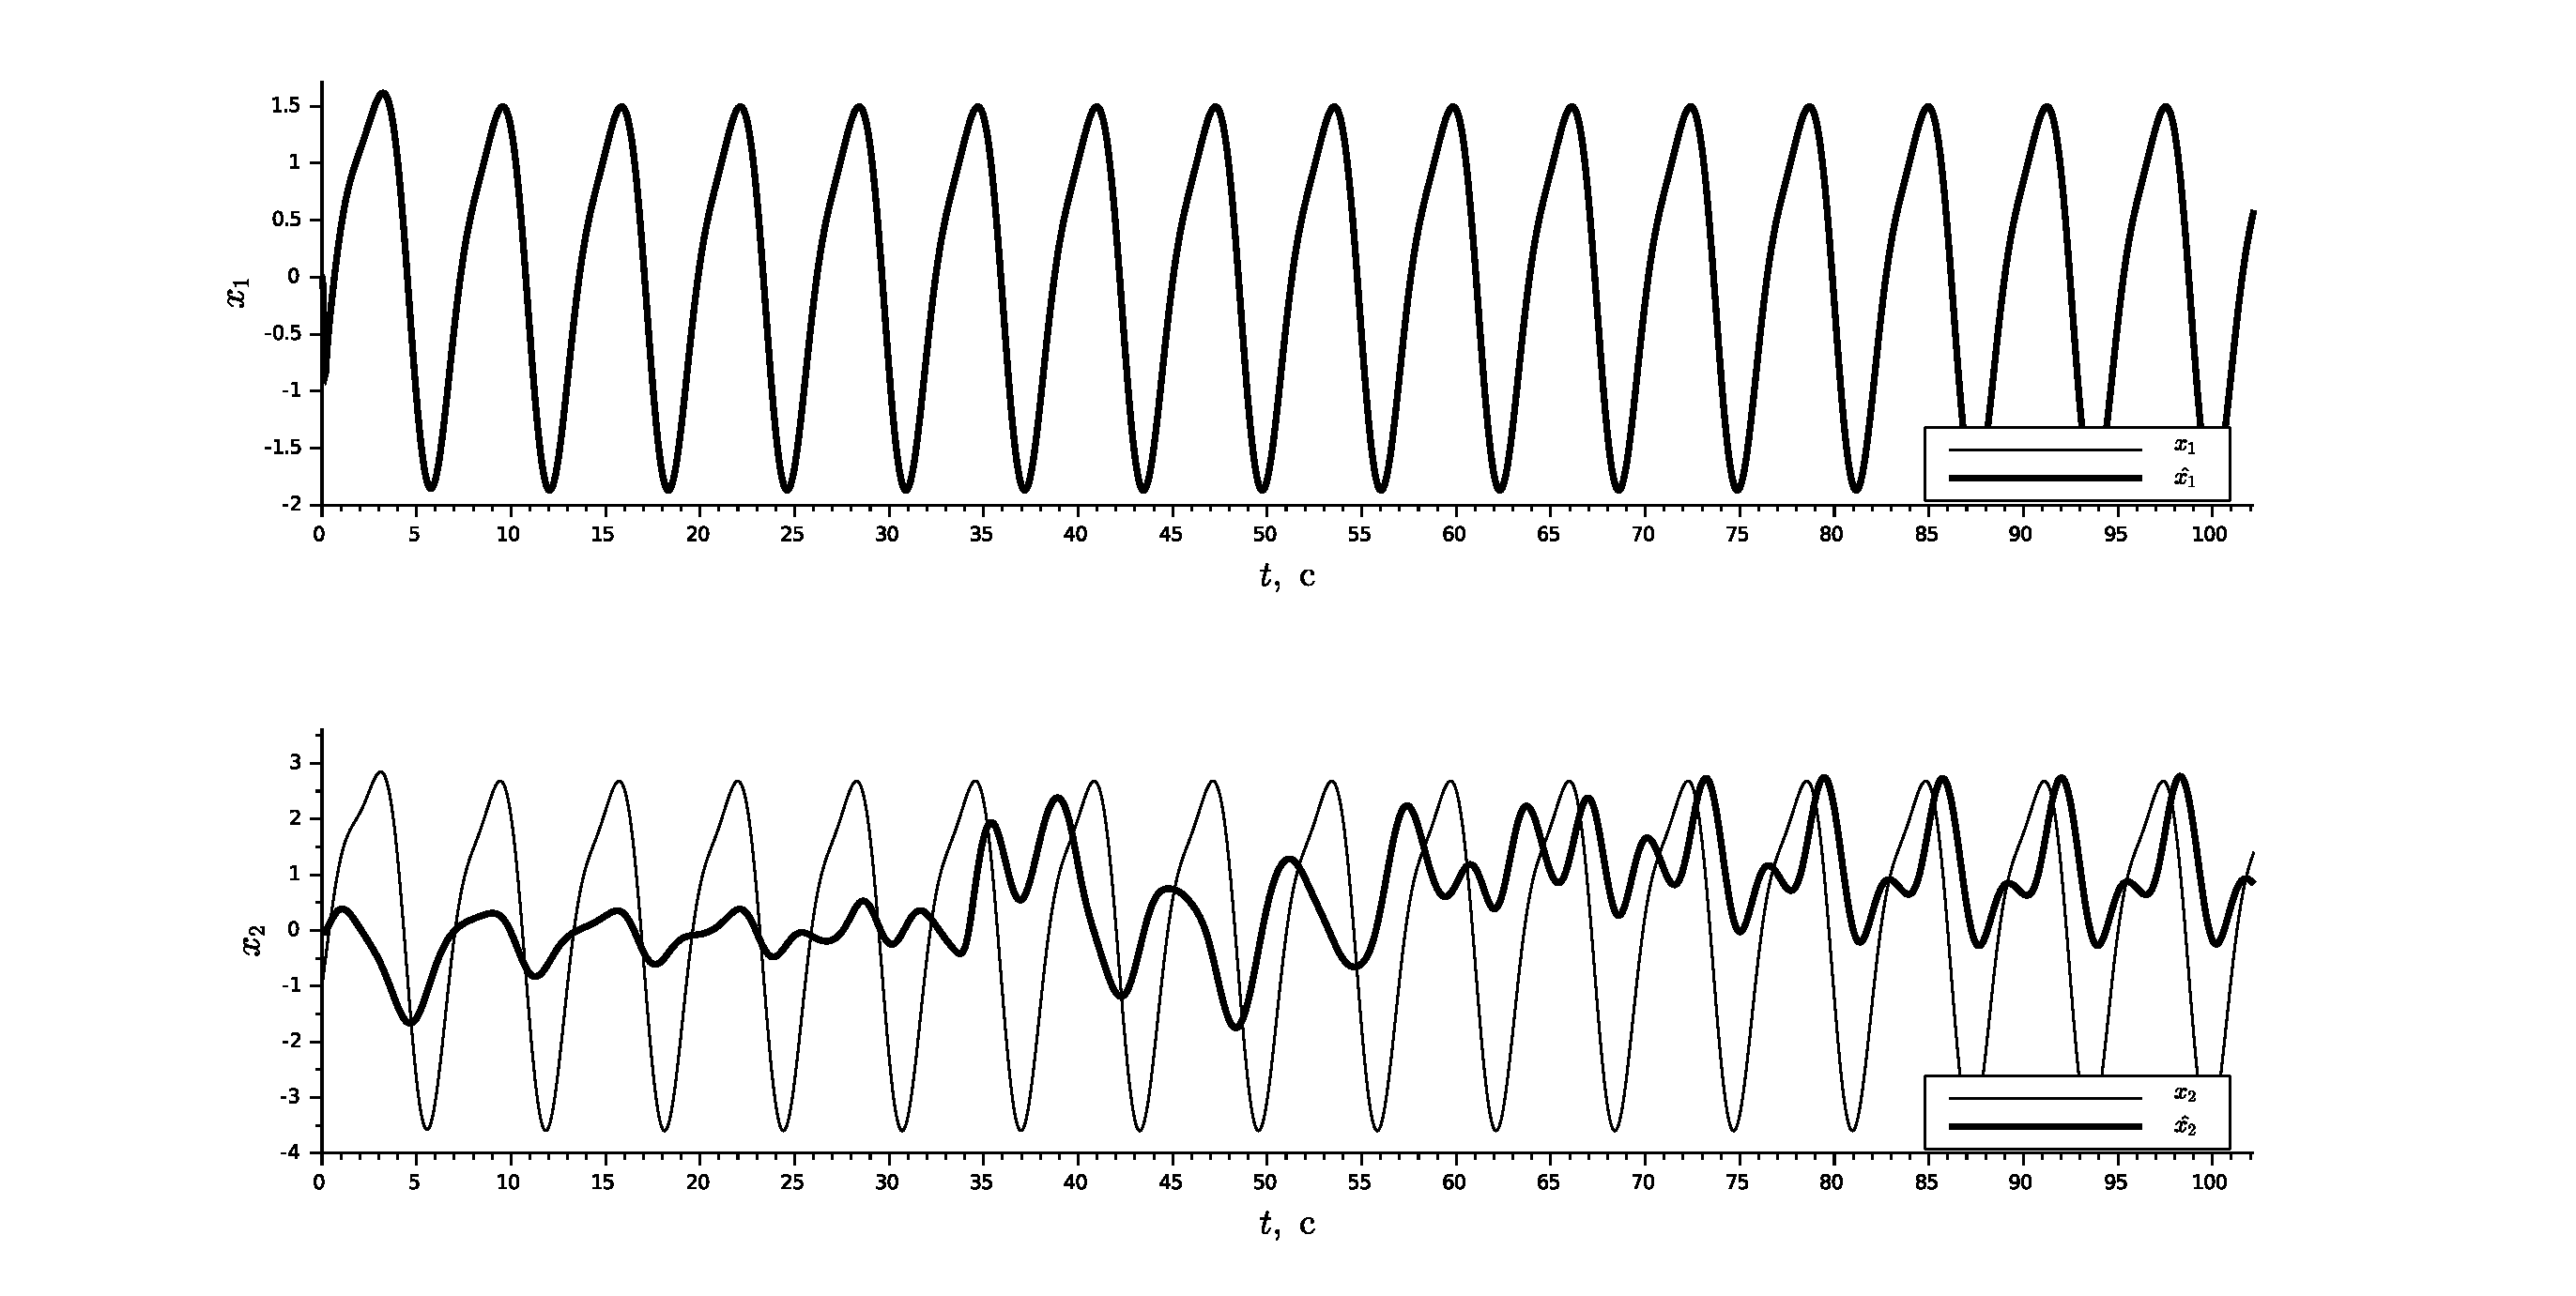
\includegraphics[width=\textwidth]{x_1_1.pdf}
    \caption{Графики компонент вектора состояния при $u = \sin{t} + 0.5 \cos{2 t}$ (0-100 секунды)}
    \label{x11}
\end{figure}

\begin{figure}[p]
	\centering
	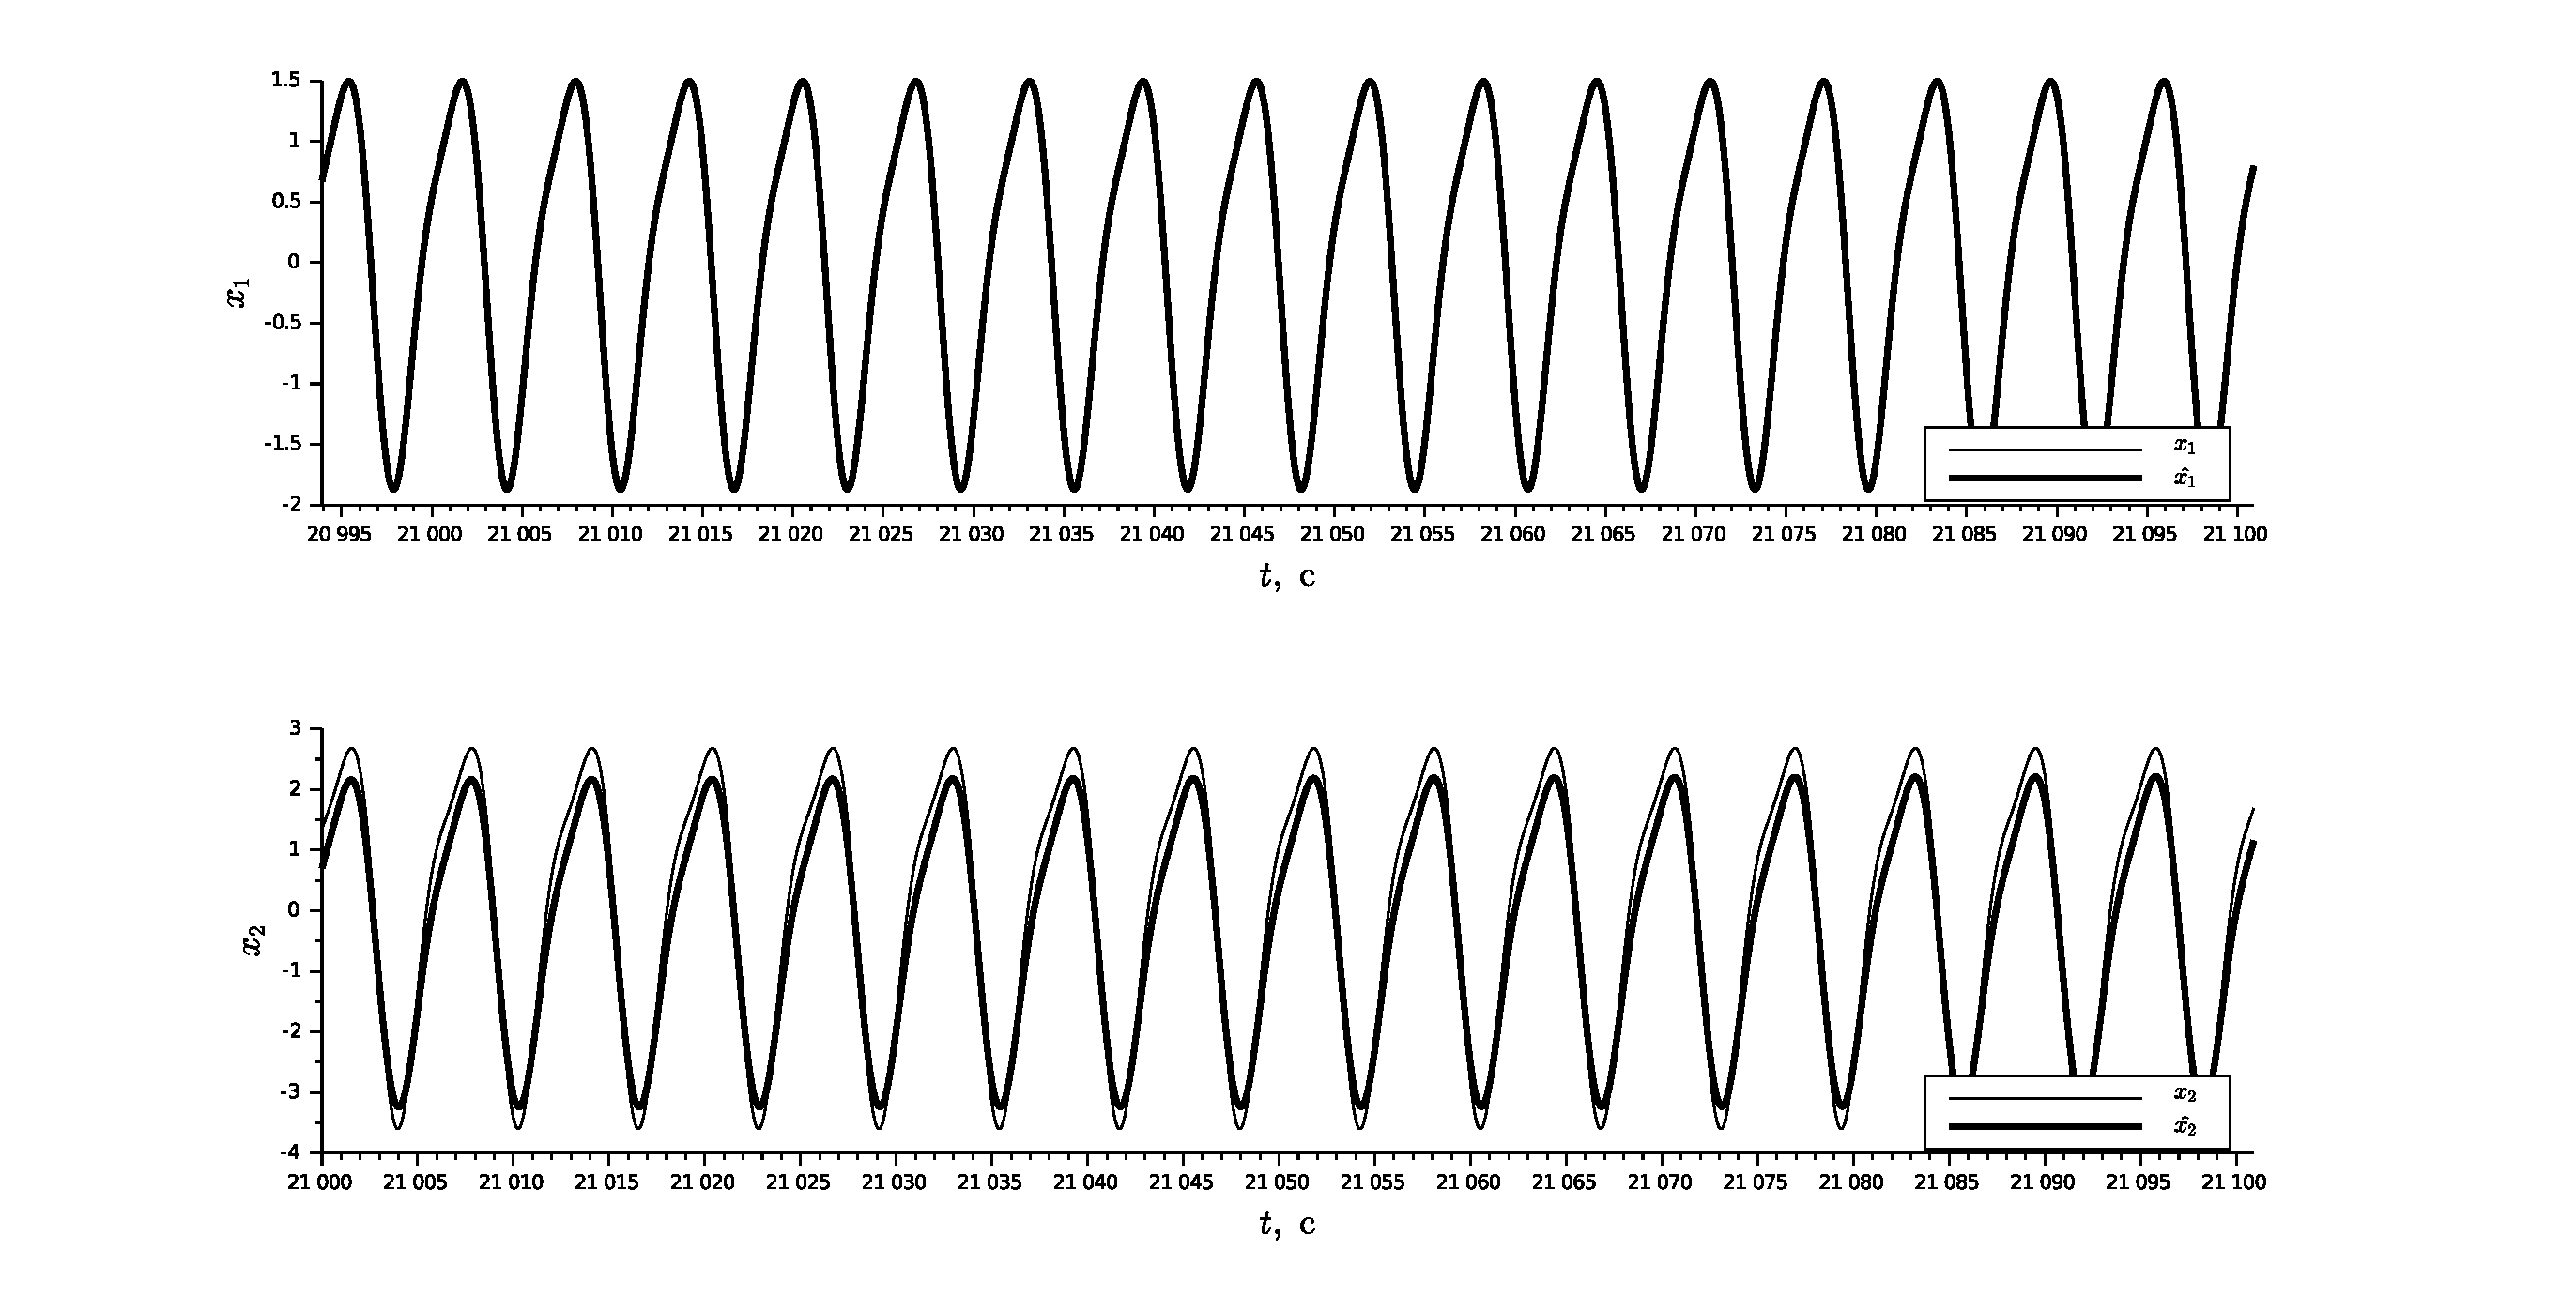
\includegraphics[width=\textwidth]{x_1_2.pdf}
	\caption{Графики компонент вектора состояния при $u = \sin{t} + 0.5 \cos{2 t}$ (21 - 21.1 тыс. секунд)}
	\label{x12}
\end{figure}

\begin{figure}[p]
	\centering
	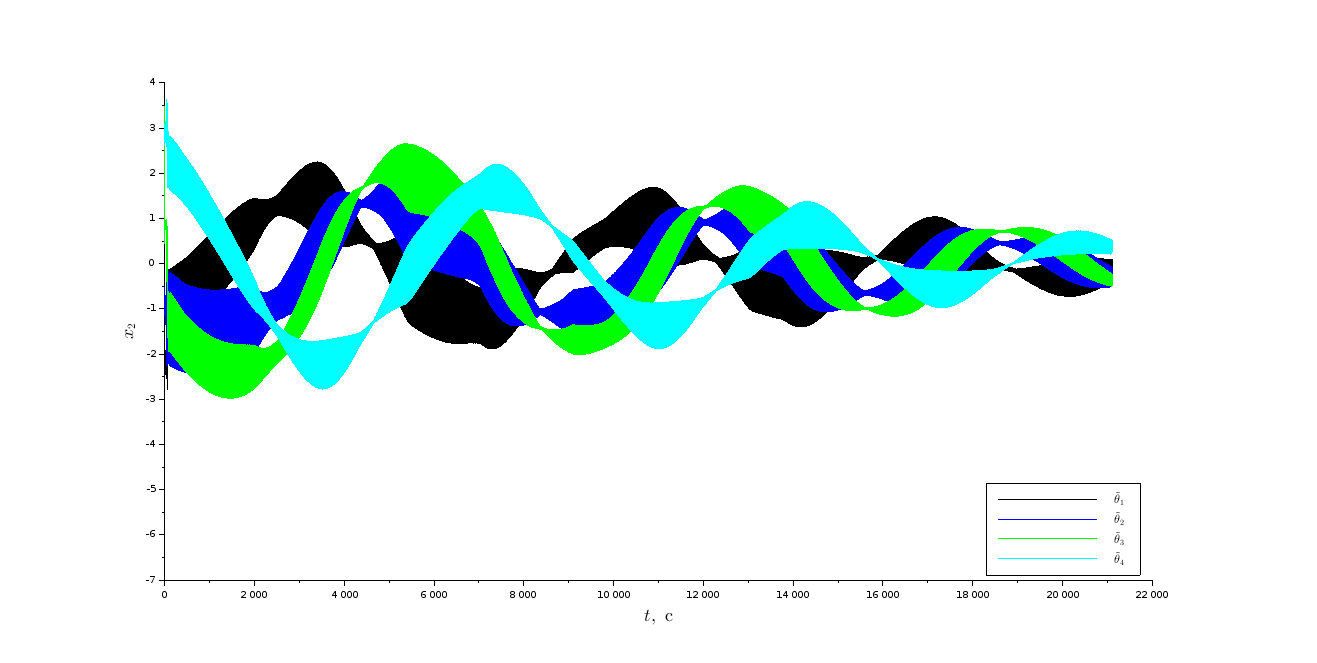
\includegraphics[width=\textwidth]{err_theta.png}
	\caption{Графики изменение параметрической ошибки при $u = \sin{t} + 0.5 \cos{2 t}$ }
	\label{err_th}
\end{figure}

\begin{figure}[p]
	\centering
	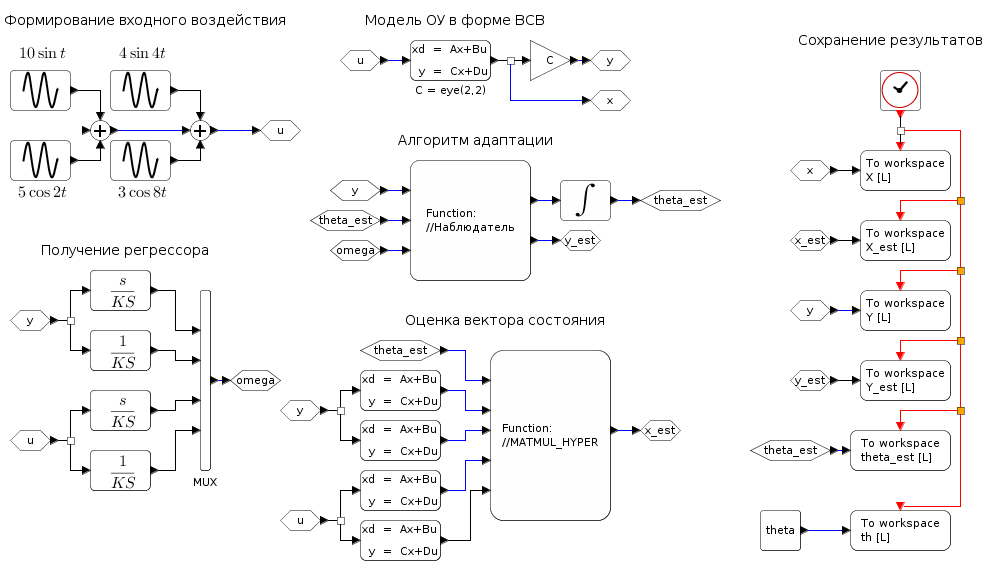
\includegraphics[width=\textwidth]{adapt_observer_2.png}
	\caption{Схема моделирования, применяемая для проверки работы адаптивного наблюдателя вектора состояния объекта ($\gamma = 1000$)}
	\label{sh2}
\end{figure}
\clearpage
\begin{figure}[p]
	\centering
	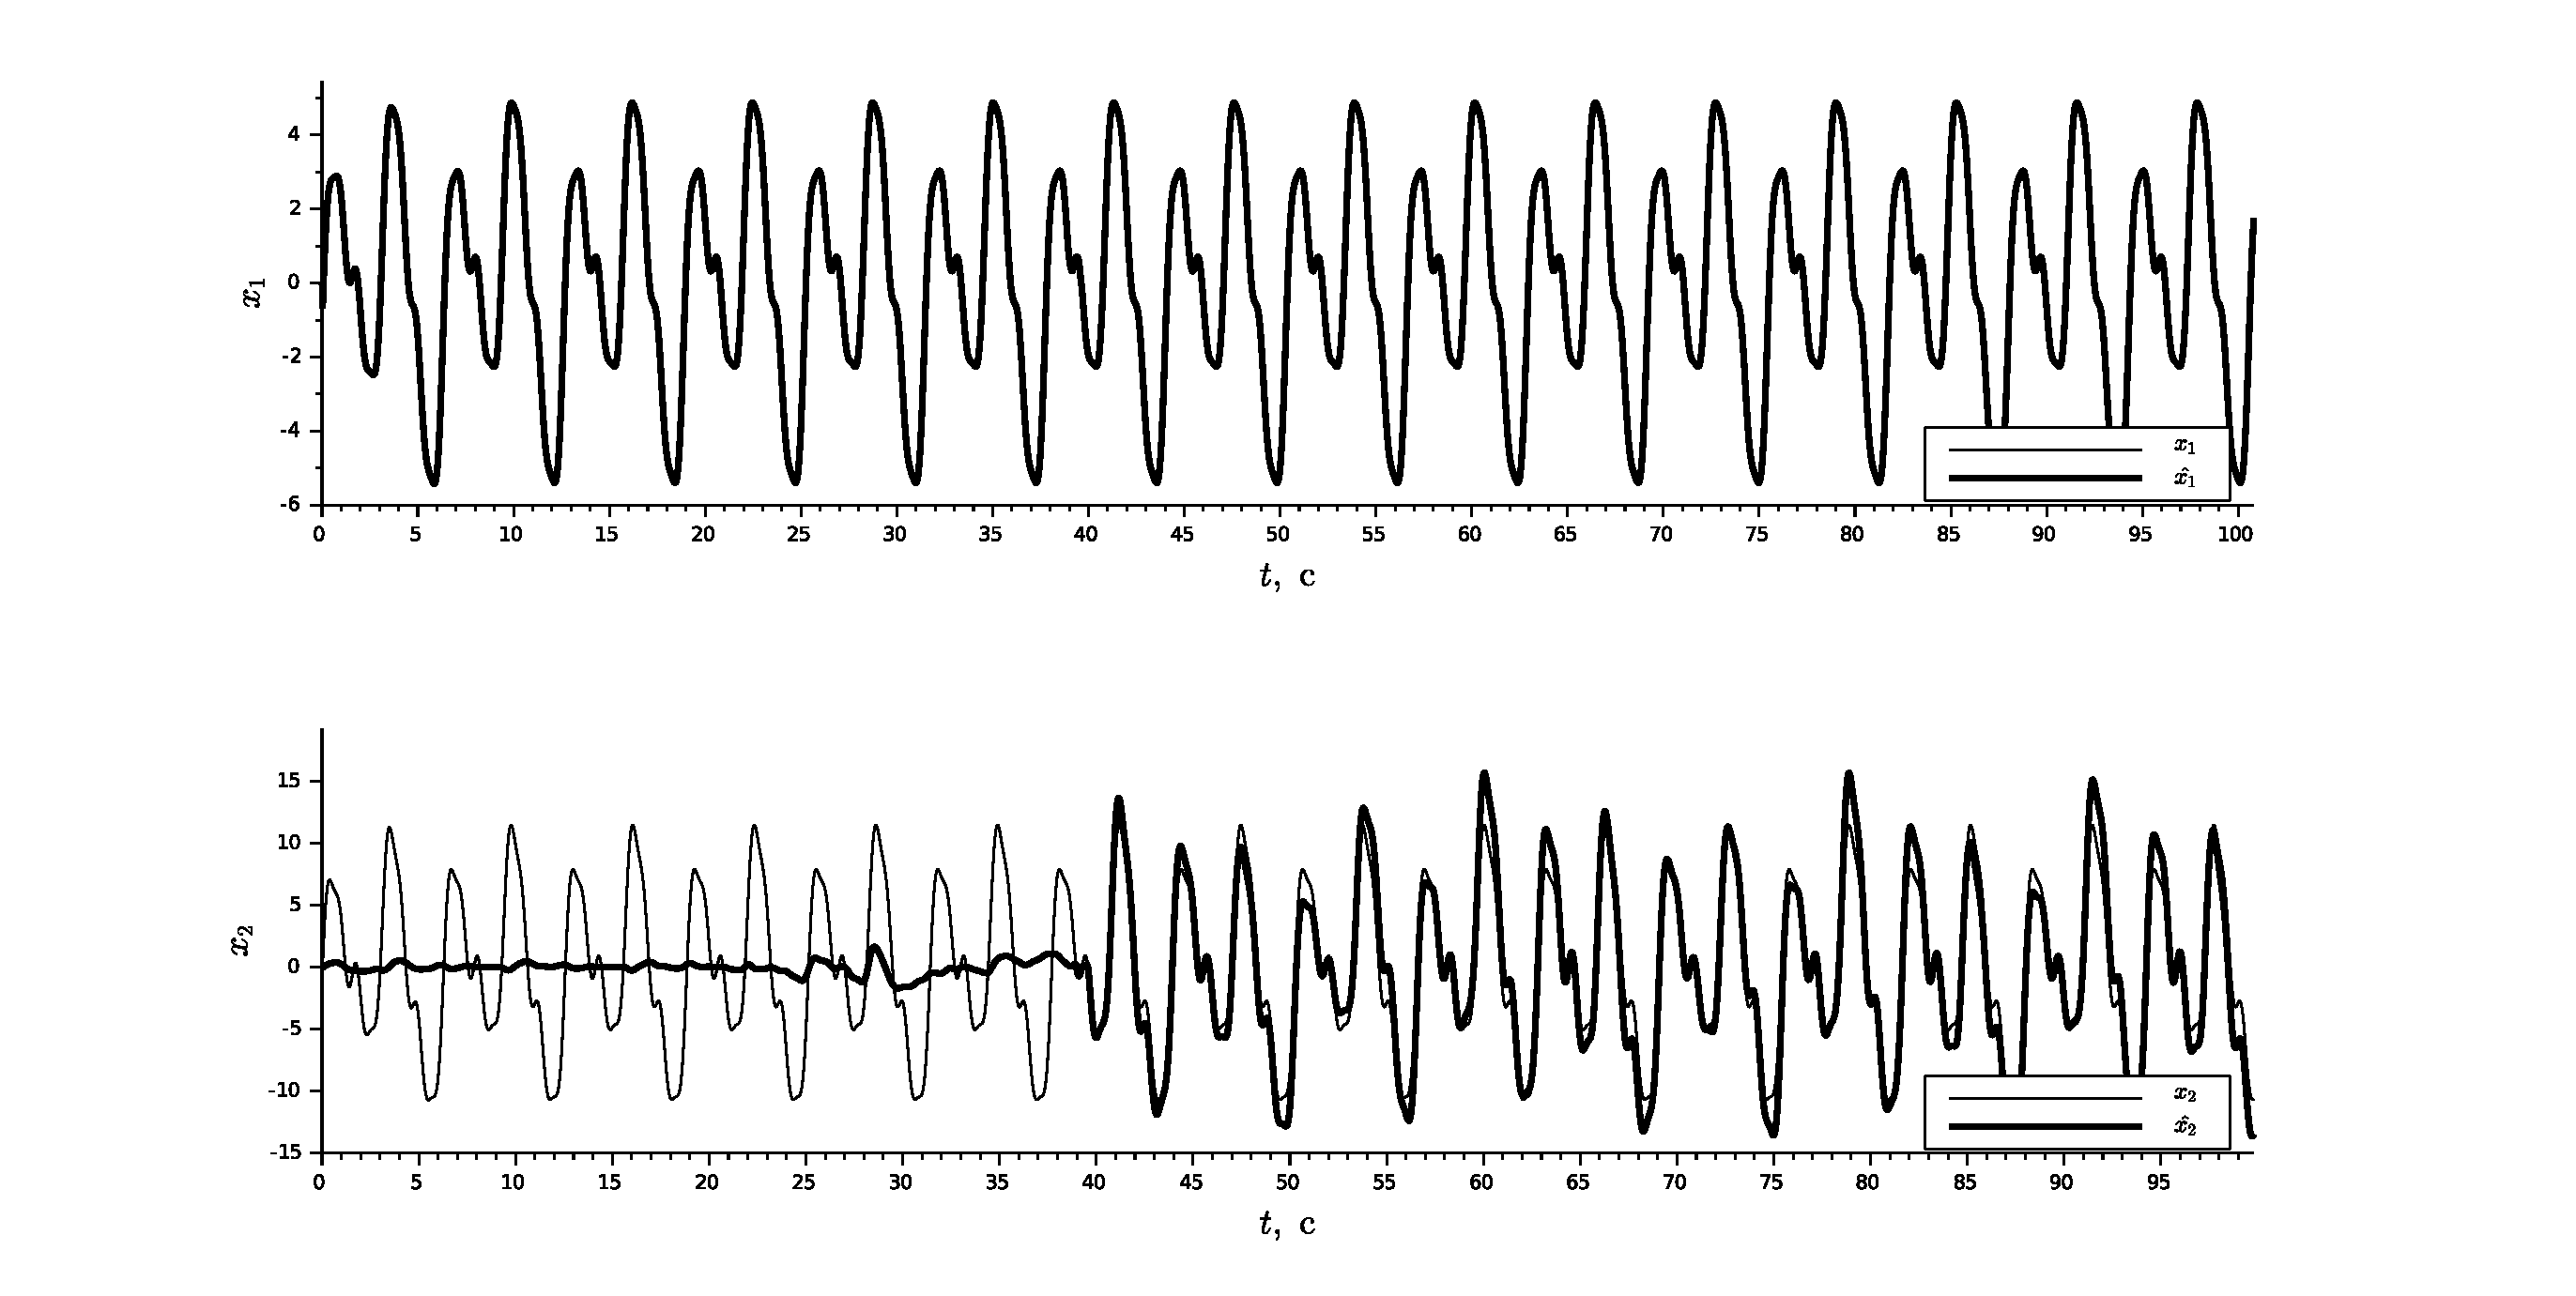
\includegraphics[width=\textwidth]{x_2_1.pdf}
	\caption{Графики компонент вектора состояния при $u = 10 \sin{t} + 5 \cos{2 t} + 4 \cos{4 t} + 3 \cos{8 t}$ (0-100 секунды)}
	\label{x21}
\end{figure}

\begin{figure}[p]
	\centering
	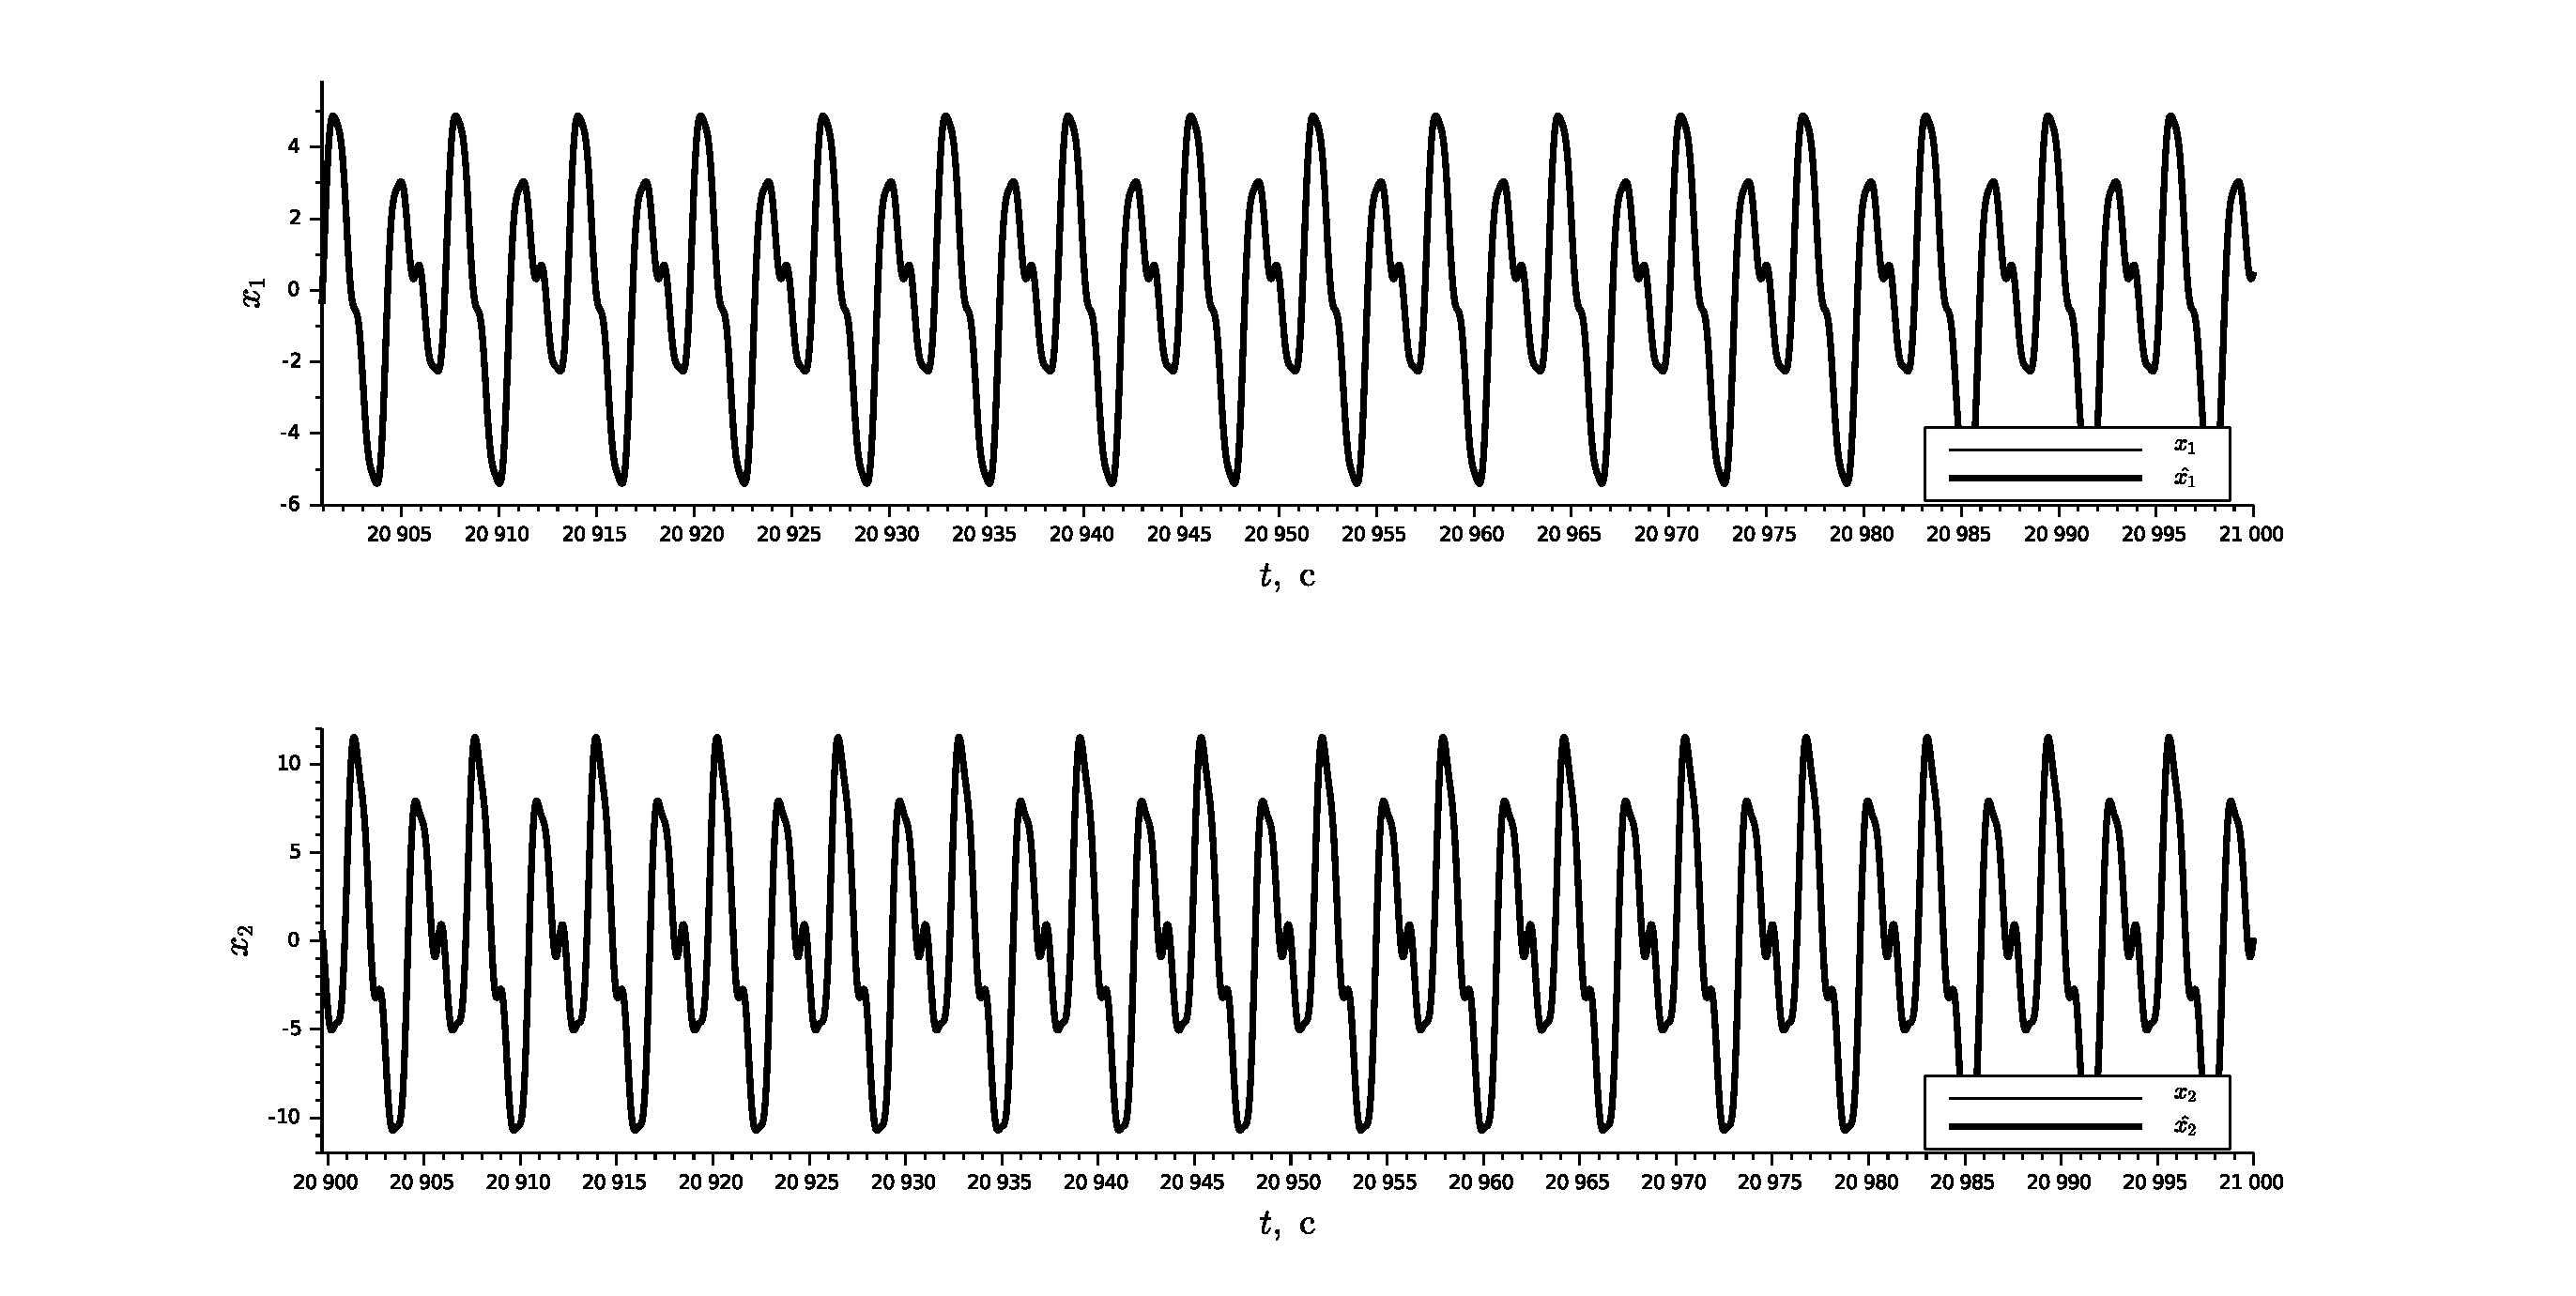
\includegraphics[width=\textwidth]{x_2_2.pdf}
	\caption{Графики компонент вектора состояния при $u = 10 \sin{t} + 5 \cos{2 t} + 4 \cos{4 t} + 3 \cos{8 t}$ (20.9 - 21 тыс. секунд)}
	\label{x22}
\end{figure}

\begin{figure}[p]
	\centering
	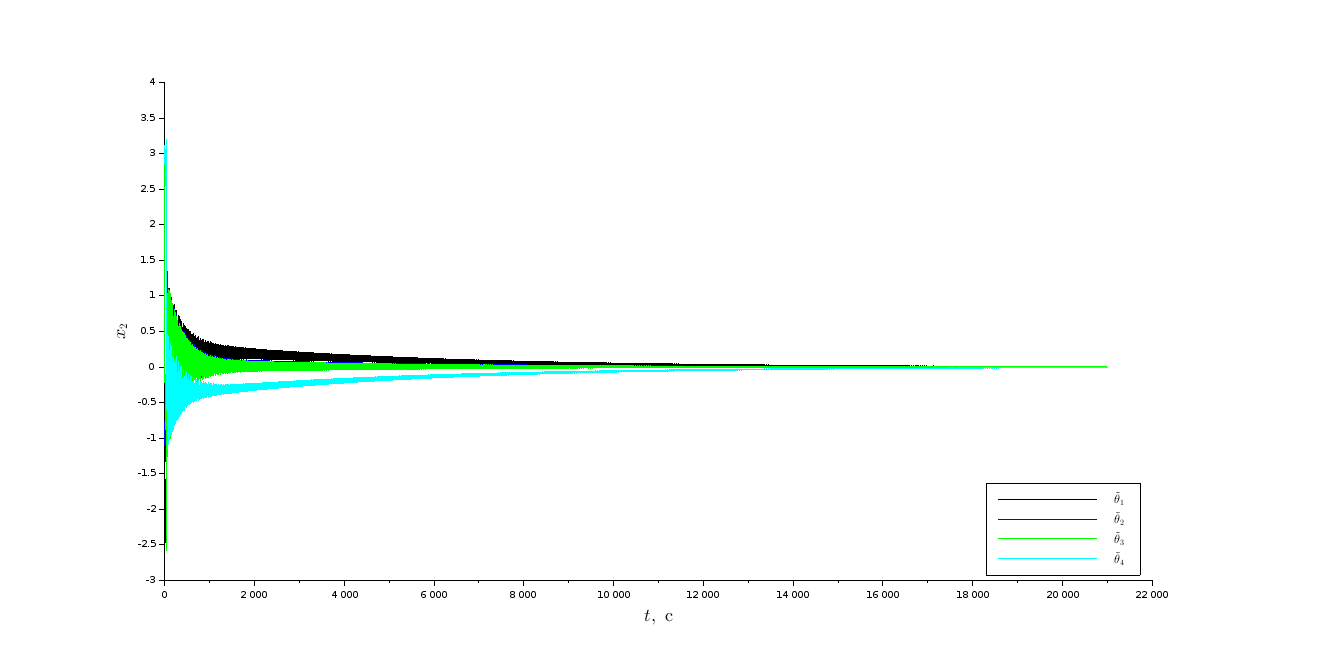
\includegraphics[width=\textwidth]{err_theta_1.png}
	\caption{Графики изменение параметрической ошибки при $u = \sin{t} + 0.5 \cos{2 t}$ }
	\label{err_th_2}
\end{figure}

\clearpage
\section{Выводы по работе}
Алгоритм адаптации \eqref{aa} обеспечивает ограниченность всех сигналов в системе, при условии ограниченного $u$ и устойчивости объекта; ошибка $\varepsilon$ стремится к нулю асимптотически; параметрические ошибки $\tilde{\theta}$ стремятся к нулю, если вектор $\omega$ удовлетворяет условию неисчезающего возбуждения; если ошибки $\tilde{\theta}$ стремятся к нулю, то оценка вектора состояния $\hat{x}$ стремится к $x$. Также было установлено, что при насыщении частотной составляющей сигнала $u$ <<достаточным>> количеством гармоник, параметрическая ошибка $\hat{\theta}$ быстрее стремится к нулю.